\documentclass{article} % For LaTeX2e
\usepackage{nips15submit_e,times}
\usepackage{hyperref}
\usepackage{url}
\usepackage{graphicx}
%\documentstyle[nips14submit_09,times,art10]{article} % For LaTeX 2.09


\title{Streaming Naive Bayes for 10605 15 Fall}


\author{
Jingyuan Liu\\
AndrewId: jingyual\\
\texttt{jingyual@andrew.cmu.edu} \\
}


\newcommand{\fix}{\marginpar{FIX}}
\newcommand{\new}{\marginpar{NEW}}


\nipsfinalcopy % Uncomment for camera-ready version


\begin{document}
\maketitle


\section{Question 1}
As the question enlights, we could use a hashmap to store the event counter. The
map key is the event key, and the value is the current counts of the key. We
could save several keys as given by the question, 10, 100, 1000, and 10000. When
the map is full, which is the key number reaches the pre-set threshold, we can
print out all items in the map. the result is as follows:\\

\begin{figure}[h]
\begin{center}
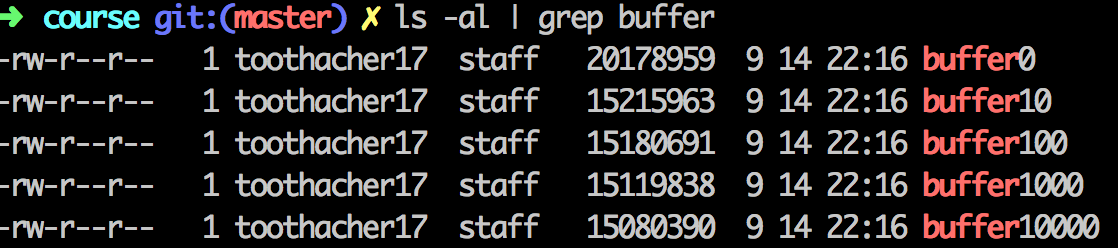
\includegraphics[width=80mm]{pic/buffer_result.png}
\end{center}
\caption{Different file size with different buffer size.}
\label{fig:buffer_result}
\end{figure}

As the Figure \ref{fig:buffer_result} shows, the buffer0 is without buffer, the
bufferX is with buffer of key size equals X. We can see that, adding buffer is
obviously outperforms the algorithm without buffer. On the other hand, the
buffer size, like 10, 100 or 10000, dose not influence much.

As far as I am concerned, the result is reasonable. Adding buffer will be of course
better than without buffer, because it collects the items with the same key and
store them in memory, thus making less printout. However, the buffer size is not
so influential as expected. I think it is that the key distribution are random,
so the map always tends to miss, just like cache miss. So the map does not
differ much with different buffer size.


\section{Question 2}
The algorithm to calculate the vocabulary size is just similar to other count
algorithms, Specifically:

1. First step: Before reading  stream data, we set a previousKey =
Null, and a totalCnt = 0.

2. Second step: For each stream instance, we parse the instance and get the current
tmpKey.

3. Third step: If the tmpKey does not equal previousKey, then totalCnt++, and set
previousKey = tmpKey. Else, pass.

4. Fourth Step: Save the totalCnt. It is the total vocabulary size.

This algorithm is able to work, because the stream data is sorted. If
it does not equal the preivous key, then it is the first time to appear,
so just add one to the totalCnt.


\section{Question 3}
The general framework is similar to Naive Bayes, but it is a little more complex
when doing the MergeCounts. It would need two previous keys record both word
information and doc information. Besides, before we know the df value of a word,
we could not print out, and we would need two lists to store the values to print
later. The general algorithm contains three major parts: ReadFile, Sort,
MergeCounts.


\subsection{ReadFile}
In this step, we just read file and produce output. Besides, considering in the
final steps we need to calculate the idf value, so we need to record the whole
doc size. We can add some ascii prefix to make sure that after sorting, the
whole size will be the first to print out.

Input: original file

Output: (wi, dj) and ds. The wi is the ith word, the dj is the jth doc, and ds
is the doc size.

\subsection{Sort}
In this step, we sort the coming stream from ReadFile step. The sorting is based
on two keys: the word and docId. Besides, the whole filesize ds will be the
first to output.

Input: (wi, dj) and ds.

Output: ds, ordered (wi, dj). The order is by the combined key wi+dj. For
example, (w1, d1), (w1, d1), (w1, d2), ...(wi,dj), (wi,dj+1), (wi+1,d1).

\subsection{MergeWord}
Merging is not only based on word key, but also related to doc key. We will
use two temp lists to store some value, however, the two temp lists will not
be big, because we just store different word and doc combinations.

Input: ds, ordered (wi, dj)

Output: (wi, dj) \quad (tf=k, idf=m)

Specific Steps:

Initialize wordPreKey, docPreKey, tfTmp = 0,
dfTmp = 0, totalSize = ds, tmpKeyList, tmpValueList

For instance in Stream:

\qquad parse instance, get wordTmpKey, docTmpKey

\qquad \qquad if wordTmpKey == wordPreviousKey:

\qquad \qquad \qquad if docTmpKey == docPreviousKey: tfTmp++

\qquad \qquad \qquad else:

\qquad \qquad \qquad \qquad tmpKeyList.add(wordPreKey+docPreKey); tmpValueList.add(tfTmp);

\qquad \qquad \qquad \qquad reset tfTmp = 0 and docPreKey = docTmpKey; dfTmp++

\qquad \qquad else:

\qquad \qquad \qquad for key, value in keyTmpList, ValueTmpList:

\qquad \qquad \qquad \qquad print \quad (key(0),key(1)) \quad (tf=value,
idf=(totalSize/dfTmp))

\qquad \qquad \qquad reinitialize everything; then set preKeys = tmpKeys

\section{Question 4}
The figure is as follows, the x is the doc size, and the y is the word size:

\begin{figure}[h]
\begin{center}
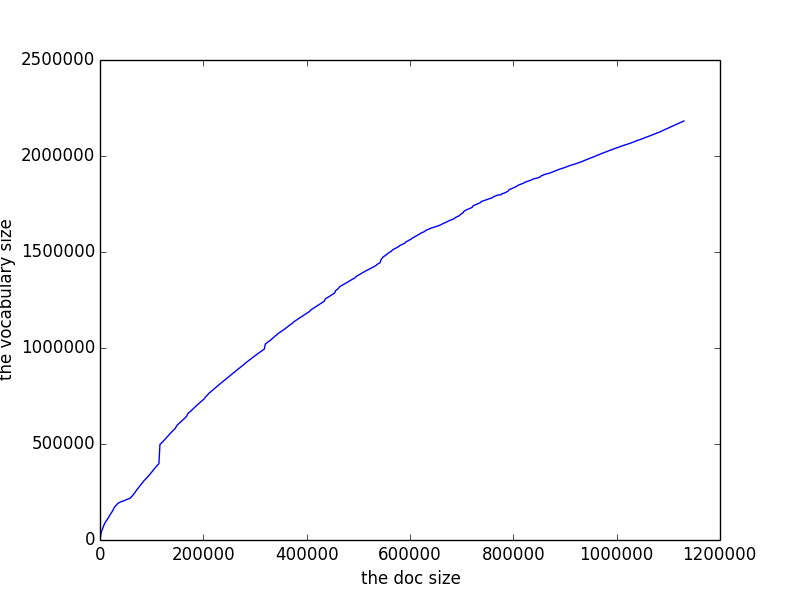
\includegraphics[width=100mm]{pic/doc_word.png}
\end{center}
\caption{The trend of word increasement over doc.}
\label{fig:doc_word}
\end{figure}

The distribution is more like a logarithmically distribution. I think it is
reasonable. As the doc size grows, the growing speed of word should decrease,
because most words may already appread before.

For validation, we can try some other distributions. We can set x as sqrt(doc
size), and y the word size. The figure is as follows:

\begin{figure}[h]
\begin{center}
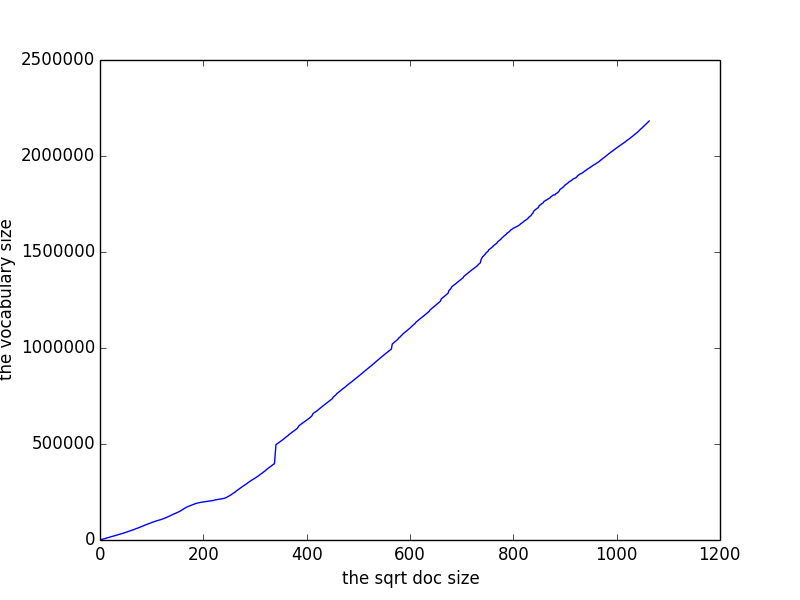
\includegraphics[width=100mm]{pic/sqrtdoc_word.png}
\end{center}
\caption{The trend of word increasement over sqrt(doc).}
\label{fig:sqrtdoc_word}
\end{figure}

As we can see from the Figure \ref{fig:sqrtdoc_word}, the doc increasement is
more linearly related over the sqrt doc increasment size, which is just as
mentioned in classes.


\end{document}
